\documentclass[12px]{article}
% \usepackage{amsmath}
\usepackage[fleqn]{amsmath}
\usepackage{amssymb}
\usepackage{graphicx}
\usepackage{cancel}
\graphicspath{ {./images/} }

\newcommand{\R}{\mathbb{R}}


\begin{document}

    \title{ECH 267 Nonlinear Control Theory \\ Homework \#1  }

    \author{Jonathan Dorsey: Department of Mechanical \& Aerospace Engineering}

    \maketitle


    \section{Problem \#1}
    Consider a single-input-single-output system described by the nth-order differential equation.

    \[ y^{(n)} = g_{1} \left(t, y, \dot{y}, ... ,y^{(n-1), u}  \right) + g_{2} \left( t, y, \dot{y}, ... ,y^{(n-2)}\right)\dot{u}   \]

    where $g_{2}$ is a differentialable function of its arguments. With $u$ as input and $y$ as output, find the state-space model. Hint: $x_{n} = y^{(n-1)} - g_{2} \left( t, y, \dot{y}, ..., y^{n-2}\right)$ \\

    \textbf{Solution:} The first step is to define the state variables and then to determine the state-space model by constructing the $n-th$ first-order ODE system as follows...\\

    State Definitions:
    \begin{flalign*}
        & x_{1} = y \\
        & x_{2} = \dot{y} \\
        & \vdots \\
        & x_{n-2} = y^{n-2} \\
        & x_{n-1} = y^{n-1}\\
        & x_{n} = y^{n-1} - g_{2} \left( t, y, \dot{y}, ..., y^{n-2}\right) \\
    \end{flalign*}

    State Derivative Definitions:
    \begin{flalign*}
        & \dot{x_{1}} = x_{2} \\
        & \dot{x_{2}} = x_{3} \\
        & \vdots \\
        & \dot{x}_{n-1} = y^{n-1}\\
        & \dot{x}_{n} = y^{n} - g_{2} \left( t, y, \dot{y}, \cdots , y^{n-2}\right)\dot{u} - \left( \frac{\partial g_2}{\partial t} + \frac{\partial g_2}{\partial x_1} \cdot \frac{\partial x_1}{\partial t} + \cdots \frac{\partial g_2}{\partial x_{n-1}} \cdot \frac{\partial x_n}{\partial t} \right) u\\
    \end{flalign*}

Where the final derivative $\dot{x}_{n}$ is found by using the chain rule on the expression for $x_{n}$, since $g_2$ is a differentiable function.

    \section{Problem \#2}

    Given the block diagram of the system, we can define the following expressions and substitute them together with the standard linear state-space model to arrive at the new closed loop state-space model, as a function of $\psi(t, y)$.


        $$\dot{x} = A x + Bu $$
        $$y = Cx + Du $$

From the block diagram, it is obvious that the control input is defined as follows.
    $$ u = r - \psi(t,y) $$

By substituting this expression for the control input, we can derive the final state-space form of...

$$  \dot{x} = Ax + B\left( r - \psi(t,y) \right) $$


    \section{Problem \#3}

    Given a linear system of the form...

    $$\dot{z} = Az + Bu $$
    $$ y = Cz $$

    \subsection{Part 3.A}

    From the Block Diagram, we can infer...

    $$ U = Sin(e)$$
    $$ e = \theta_{i} - \theta_{0}$$
    $$\dot{e} = \dot{\theta_{i}} - \dot{\theta_{0}}$$

    \noindent Since $\dot{\theta_{i}}$ is constant, its derivative is zero.

    $$ \dot{e} =  - \dot{\theta_{0}} $$
    $$ \dot{\theta}_{0} = \int y dt $$
    $$ y = \dot{\theta_{0}} $$

    Therefore:

    $$ y = \dot{-e} $$

    Via substitution

    $$ \dot{z} = Az + BSin(e) $$
    $$ -\dot{e} = Cz $$

    Which matches the form of the solution given in the problem statement.



    \subsection{Part 3.B}

    For the scalar state-space realization, the equilibrium parts are acheived by setting the rate of the state equal to zero and solving for the solutions which satisfy the expression.

    $$ 0 = Az + BSin(e)$$
    $$ 0 = -Cz $$

    By simplifying the expression we achieve...

    $$ z = -A^{-1}B \cdot Sin(e)$$

    Via substitution into the output equation...

    $$ 0 = C \left( -A^{-1}B \cdot Sin(e) \right) $$

    Which can be written in generally as the plant transfer function multiplied by the sine input from the reference error.

    $$ G(t) \cdot Sin(e) = 0 $$

    Due to the initial condition $G(0) \neq 0 $, we know that the previous equation can only be valid when sine identically equals zero. $ Sin(e) = 0 $. Due to the periodic nature of the sine function we can demonstrate that...

    $$ e = 0, 2\pi, \cdots, n\pi $$
    Therefore the Equilibrium points are given by the following expression.
    $$ e = \pm n \pi$$


    \subsection{Part 3.C}

    For $G(s) = \frac{1}{\tau s + 1}$, the closed loop can be written in state-space form such that A = $-1/\tau$, B = $1/\tau$, and C = 1.

    This leads to the state-space equation...

    $$ \dot{z} = -\frac{1}{\tau}z + \frac{1}{\tau} \cdot Sin(e)  $$
    $$ \dot{e} = -z $$

    Which can further be constructed into an Augemented State-Space Via the following state definitions.

    $$ x_{1} = e $$
    $$ x_{2} = -z $$

    And constructed as follows.

    $$ \dot{x_1} = x_{2} $$
    $$ \dot{x_2} = - \frac{1}{\tau} x_2 - \frac{1}{\tau} sin(x_1)$$

    Which is the state space representation of the pendulum equation.













    \section{Problem \#4}

    Consider the mass-spring system shown in Figure 3. Assuming a linear spring and nonlinear viscous damping described by $ c_{1}\dot{y} + c_{2}\dot{y}|\dot{y}|$, find a state equation that describes the motion of the system. \\



    \textbf{Solution:} The force of linear spring is $F_{s} = kX$, the force of gravity is $ W=mg$, and the force due to damping is provided in the problem statement. By using Newton's second law, we can combine these quantities in a force balance as follows, given the mass $m$, the spring constant $k$, the acceleration due to gravity $g$, and finally the damping constants $C_{1}$ and $ C_{2}$.

    $$ m\ddot{y} = k*y + c_{1}\dot{y} + c_{2}\dot{y}|\dot{y}| -mg $$

    Given the state variables $x_{1} \& x_{2}$ defined as follows...

    \[ x_{1} = y \]
    \[ x_{2} = \dot{y} \]

    We arrive at the following state space equation...

    \[ \dot{x_{1}} = x_{2}\]
    \[ \dot{x_{2}} = \left( \frac{k}{m} \right)x_{1}  + \left[ c_{1}x_{2} + c_{2}x_{2}|x_{2}| \right]  \left( \frac{1}{m} \right) -g \]

    \section{Problem \#5}

    Given the following equation over $[0, \infty]$...

    $$
    \dot{x}(t) = [x(t)]^{\frac{1}{3}} \hspace{.3cm}, x(0) =0\\
    $$

    We can show that this problem has a \textbf{NOT unique} solution, via the ``Existance and Uniqueness Theorem''. \\

    \noindent This theorem states that if the function and its derivative are continuous around the initial condition of the system that there exists a unique solution. \\

    \noindent $\dot{x} = f(x)$ is a continuous function on the inteveral specified, however, when taking the derivative of the function $f(x)$, we note that it is \textbf{not} continuous at $x=0$ where the function become undefined.



    \section{Problem \#6}
    For each of the following systems, find all equilibrium points and determine the type of each isloated equilibrium.

    \subsection{}


    \begin{flalign*}
        & \dot{x}_{1} = x_{2} \\
        & \dot{x}_{2} = -x_{1} + \frac{x^{3}_{1}}{6} -x_{2}\\
    \end{flalign*}

    We can determine the equilibrium points of the system by setting the state equations equal to zero and solving.

    \begin{flalign*}
        & 0 = x_{2} \\
        & 0 = -x_{1} + \frac{x^{3}_{1}}{6} -x_{2}\\
    \end{flalign*}

    Which yields the following equilibrium points.

    \begin{flalign*}
        & P_{1} = (0,0) \\
        & P_{2} = (\sqrt{6}, 0 ) \\
        & P_{3} = (-\sqrt{6}, 0 ) \\
    \end{flalign*}

    These equilibria can be used to derive a linearized system to indentify the `type' of the equilibrium point.

    $$
    \begin{matrix}
        & \frac{\partial f_{1}}{\partial x_{1}} = 0 & \frac{\partial f_{1}}{\partial x_{2}} = 1 \\
        & \frac{\partial f_{2}}{\partial x_{1}} = \left( -1 + \frac{3x_{1}^{2}}{6} \right) & \frac{\partial f_{2}}{\partial x_{2}} = -1
    \end{matrix}
    $$

    Therefore for $P_1$, we can define the jacobian matrix $A_j$ as ...

    $$ A_j =
    \begin{bmatrix}
        0 & 1 \\
        -1 & -1
    \end{bmatrix}\Big|_{P_1}
    $$

    where the eigenvalues of the linearized system are $\lambda_{P_{1}} = -.5 \pm .866j$. Therefore the linearization of this system about $P_1$ yields a \textbf{Stable Focus}.


Therefore for $P_2$, we can define the jacobian matrix $A_j$ as ...

$$ A_j =
\begin{bmatrix}
    0 & 1 \\
    2 & -1
\end{bmatrix}\Big|_{P_2}
$$

where the eigenvalues of the linearized system are $\lambda_{P_{2}} = 1, -2$. Therefore the linearization of this system about $P_2$ yields a \textbf{saddle point}.

In a similar manner for $P_3$, we can define the jacobian matrix $A_j$ as ...

$$ A_j =
\begin{bmatrix}
    0 & 1 \\
    2 & -1
\end{bmatrix}\Big|_{P_3}
$$

where the eigenvalues of the linearized system are $\lambda_{P_{3}} = 1, -2$. Therefore the linearization of this system about $P_3$ yields a \textbf{saddle point}.










    \subsection{}

    \[ \dot{x}_{1} = -x_{1} + x_{2}\]
    \[  \dot{x}_{2} = 0.1x_{1} - 2x_{2} - x_{1}^{2} - 0.1x_{1}^{3}\]

    We can determine the equilibrium points of the system by setting the state equations equal to zero and solving.

    \begin{flalign*}
        & 0 =-x_{1} + x_{2} \\
        & 0 = 0.1x_{1} - 2x_{2} - x_{1}^{2} - 0.1x_{1}^{3}\\
    \end{flalign*}

    Which yields the following equilibrium points.

    \begin{flalign*}
        & P_{1} = (0,0) \\
        & P_{2} = (x_1, x_2 = -7.44949 ) \\
        & P_{3} = (x_1, x_2 = -2.55051) \\
    \end{flalign*}

    These equilibria can be used to derive a linearized system to indentify the `type' of the equilibrium point.

    $$
    \begin{matrix}
        & \frac{\partial f_{1}}{\partial x_{1}} = -1 & \frac{\partial f_{1}}{\partial x_{2}} = 1 \\
        & \frac{\partial f_{2}}{\partial x_{1}} = \left( .1 - 2x_{1} -.3x_{1}^2 \right) & \frac{\partial f_{2}}{\partial x_{2}} = -2
    \end{matrix}
    $$

    Therefore for $P_1$, we can define the jacobian matrix $A_j$ as ...

    $$ A_j =
    \begin{bmatrix}
        -1 & 1 \\
        .1 & -2
    \end{bmatrix}\Big|_{P_1}
    $$

    where the eigenvalues of the linearized system are $\lambda_{P_{1}} = -.9084, -2.0916$. Therefore the linearization of this system about $P_1$ yields a \textbf{Stable Node}.


    Therefore for $P_2$, we can define the jacobian matrix $A_j$ as ...

    $$ A_j =
    \begin{bmatrix}
    -1 & 1 \\
    1.6494 & -2
    \end{bmatrix}\Big|_{P_2}
    $$

    where the eigenvalues of the linearized system are $\lambda_{P_{2}} = -.1218, -2.8782$. Therefore the linearization of this system about $P_2$ yields a \textbf{Stable Node}.

    In a similar manner for $P_3$, we can define the jacobian matrix $A_j$ as ...

    $$ A_j =
    \begin{bmatrix}
    -1 & 1 \\
    3.2494 & -2
    \end{bmatrix}\Big|_{P_3}
    $$

    where the eigenvalues of the linearized system are $\lambda_{P_{3}} = .3707, -3.3707 $. Therefore the linearization of this system about $P_3$ yields a \textbf{saddle point}.


    \subsection{}

    \[ \dot{x}_{1} = (1-x_1)x_1 - \frac{2x_{1}x_{2}}{1 + x_1} \]
    \[  \dot{x}_{2} = \left( 2 - \frac{x_{2}}{1 + x_{1}} \right) x_{2}\]


    We can determine the equilibrium points of the system by setting the state equations equal to zero and solving.

    \begin{flalign*}
        & 0 = (1-x_1)x_1 - \frac{2x_{1}x_{2}}{1 + x_1} \\
        & 0 = \left( 2 - \frac{x_{2}}{1 + x_{1}} \right) x_{2}\\
    \end{flalign*}

    Which yields the following equilibrium points.

    \begin{flalign*}
        & P_{1} = (0,0) \\
        & P_{2} = (x_1 = -3, x_2 = -4 ) \\
    \end{flalign*}

    These equilibria can be used to derive a linearized system to indentify the `type' of the equilibrium point.

    Therefore for $P_1$, we can define the jacobian matrix $A_j$ as ...

    $$ A_j =
    \begin{bmatrix}
        1 & 0 \\
        0 & 2
    \end{bmatrix}\Big|_{P_1}
    $$

    where the eigenvalues of the linearized system are $\lambda_{P_{1}} = 1, 2$. Therefore the linearization of this system about $P_1$ yields a \textbf{Unstable Node}.


    Therefore for $P_2$, we can define the jacobian matrix $A_j$ as ...

    $$ A_j =
    \begin{bmatrix}
    9 & -3 \\
    -4 & -2
    \end{bmatrix}\Big|_{P_2}
    $$

    where the eigenvalues of the linearized system are $\lambda_{P_{2}} = 10, -3$. Therefore the linearization of this system about $P_2$ yields a \textbf{Saddle Point}.

    \subsection{}

    \[ \dot{x}_{1} = x_{2}\]
    \[  \dot{x}_{2} = -x_{1} + x_{2} \left( 1 - 3x_{1}^{2} -2x_{2}^{2} \right)\]


    We can determine the equilibrium points of the system by setting the state equations equal to zero and solving.

    \begin{flalign*}
        & 0 = x_{2} \\
        & 0 = -x_{1} + x_{2} \left( 1 - 3x_{1}^{2} -2x_{2}^{2} \right)\\
    \end{flalign*}

    Which yields the following equilibrium points.

    \begin{flalign*}
        & P_{1} = (0,0) \\
    \end{flalign*}

    These equilibria can be used to derive a linearized system to indentify the `type' of the equilibrium point.

    $$
    \begin{matrix}
        & \frac{\partial f_{1}}{\partial x_{1}} = 0 & \frac{\partial f_{1}}{\partial x_{2}} = 1 \\
        & \frac{\partial f_{2}}{\partial x_{1}} = \left( -1 -6x_{2}x_{1} \right) & \frac{\partial f_{2}}{\partial x_{2}} = \left(1 -3x_{1}^2 -6x_2^2 \right)
    \end{matrix}
    $$


    Therefore for $P_1$, we can define the jacobian matrix $A_j$ as ...

    $$ A_j =
    \begin{bmatrix}
        1 & 1 \\
        -1 & 1
    \end{bmatrix}\Big|_{P_1}
    $$

    where the eigenvalues of the linearized system are $\lambda_{P_{1}} = .5 \pm .866j$. Therefore the linearization of this system about $P_1$ yields a \textbf{Saddle Point}.

    \subsection{}

    \[ \dot{x}_{1} = -x_{1} + x_{2}(1 + x_{2})\]
    \[  \dot{x}_{2} = -x_{1}(1 + x_{1})\]


    We can determine the equilibrium points of the system by setting the state equations equal to zero and solving.

    \begin{flalign*}
        & 0 = -x_{1} + x_{2}(1 + x_{2}) \\
        & 0 = -x_{1}(1 + x_{1})\\
    \end{flalign*}

    Which yields the following equilibrium points.

    \begin{flalign*}
        & P_{1} = (0,0) \\
    \end{flalign*}

    These equilibria can be used to derive a linearized system to indentify the `type' of the equilibrium point.

    $$
    \begin{matrix}
        & \frac{\partial f_{1}}{\partial x_{1}} = -1 + x_2 & \frac{\partial f_{1}}{\partial x_{2}} = 1 + x_1 \\
        & \frac{\partial f_{2}}{\partial x_{1}} = -1 -2x_1 & \frac{\partial f_{2}}{\partial x_{2}} = 0
    \end{matrix}
    $$


    Therefore for $P_1$, we can define the jacobian matrix $A_j$ as ...

    $$ A_j =
    \begin{bmatrix}
        -1 & 1 \\
        -1 & 0
    \end{bmatrix}\Big|_{P_1}
    $$

    where the eigenvalues of the linearized system are $\lambda_{P_{1}} = -5 \pm .866j$. Therefore the linearization of this system about $P_1$ yields a \textbf{Stable Focus}.

    \subsection{}

    \[ \dot{x}_{1} = (x_1 - x_2) \left( x_{1}^{2} + x_{2}^{2} - 1 \right)\]
    \[  \dot{x}_{2} = (x_1 + x_2) \left( x_{1}^{2} +  x_{2}^{2} - 1 \right)\]

    We can determine the equilibrium points of the system by setting the state equations equal to zero and solving.

    \begin{flalign*}
        & 0 = (x_1 - x_2) \left( x_{1}^{2} + x_{2}^{2} - 1 \right)\\
        & 0 = = (x_1 + x_2) \left( x_{1}^{2} +  x_{2}^{2} - 1 \right)\\
    \end{flalign*}

    Which yields the following equilibrium points.

    \begin{flalign*}
        & P_{1} = (0,0) \\
    \end{flalign*}

    These equilibria can be used to derive a linearized system to indentify the `type' of the equilibrium point.

    Therefore for $P_1$, we can define the jacobian matrix $A_j$ as ...

    $$ A_j =
    \begin{bmatrix}
        -1 & 1 \\
        -1 & -1
    \end{bmatrix}\Big|_{P_1}
    $$

    where the eigenvalues of the linearized system are $\lambda_{P_{1}} = -1 \pm 1j$. Therefore the linearization of this system about $P_1$ yields a \textbf{Stable Focus}.

    \subsection{}

    \[ \dot{x}_{1} = -x_{1}^{3} + x{2}\]
    \[  \dot{x}_{2} = x_{1} - x_{2}^{3}\]


    We can determine the equilibrium points of the system by setting the state equations equal to zero and solving.

    \begin{flalign*}
        & 0 = -x_{1}^{3} + x{2} \\
        & 0 = x_{1} - x_{2}^{3}\\
    \end{flalign*}

    Which yields the following equilibrium points.

    \begin{flalign*}
        & P_{1} = (0,0) \\
        & P_{2} = (x_2= x_1 = 1) \\
        & P_{3} = (x_2= x_1 = -1) \\
    \end{flalign*}

    These equilibria can be used to derive a linearized system to indentify the `type' of the equilibrium point.

    $$
    \begin{matrix}
        & \frac{\partial f_{1}}{\partial x_{1}} = -3x_1^{2} & \frac{\partial f_{1}}{\partial x_{2}} = 1 \\
        & \frac{\partial f_{2}}{\partial x_{1}} = 1 & \frac{\partial f_{2}}{\partial x_{2}} = -3x_2^{2}
    \end{matrix}
    $$


    Therefore for $P_1$, we can define the jacobian matrix $A_j$ as ...

    $$ A_j =
    \begin{bmatrix}
        0 & 1 \\
        1 & 0
    \end{bmatrix}\Big|_{P_1}
    $$

    where the eigenvalues of the linearized system are $\lambda_{P_{1}} = -1, 1$. Therefore the linearization of this system about $P_1$ yields a \textbf{Saddle Point}.

    Therefore for $P_2$ \& $P_3$, we can define the jacobian matrix $A_j$ as ...

    $$ A_j =
    \begin{bmatrix}
        -3 & 1 \\
        1 & -3
    \end{bmatrix}\Big|_{P_2 \: or \: P_3}
    $$

    where the eigenvalues of the linearized system are $\lambda_{P_{2}} = \lambda_{P_{3}} = -4, -2$. Therefore the linearization of this system about $P_2$ and $P_3$ yields a \textbf{Stable Node}.


\section{Problem \# 7}

\begin{itemize}
    \item (a): Determine the matrix M that transforms A into the appropriate modal form and write the system in model coordinates.
    \item (b): Classify the equilibrium (0, 0)
    \item (c): Generate the Phase Portrais of the system in both modal(z) and original(x) coordinates.

\end{itemize}

\subsection*{Part 7.A}
In order to determine the matrix M such that $\dot{z} = \left(M^{-1}AM \right)z$, for each of the matrices in the problem statement, such that the problem will be transformed into modal coordinates, we must first compute the eigenvalues and eigenvectors for each matrix. We can then compute the M matrix by concatenating the eigenvectors of the given matrix A, and finally we can find $M^{-1}$ by taking the matrix inverse of the M previously derived. By following these steps, we can transform A into its modal form. \\

To accomplish this, I utilized MATLAB to compute the eignvalues and eigenvectors, even though for these simple 2x2 matrices would be simple enough to compute by hand. However, these calculations would have been time consumming.

\subsubsection*{7.A.i}

Eigenvalue:
$$ \lambda = -1, -2 $$
Eigenvector:
$$M =
\begin{bmatrix}
    & .7071 & -.4472 \\
    & -.7071 & .8944
\end{bmatrix}
$$


\subsubsection*{7.A.ii}

Eigenvalue:
$$ \lambda = 1, 1 $$
Eigenvector:
$$M =
\begin{bmatrix}
    & -.7071 & -.7071 \\
    & .7071 & .7071
\end{bmatrix}
$$
\subsubsection*{7.A.iii}

Eigenvalue:
$$ \lambda = -1, 1 $$
Eigenvector:
$$M =
\begin{bmatrix}
    & 1 & -.4472 \\
    & 0 & .8944
\end{bmatrix}
$$
\subsubsection*{7.A.iv}

Eigenvalue:
$$ \lambda = \pm2j $$
Eigenvector:
$$M =
\begin{bmatrix}
    & .9129 & .9129 \\
    & -.1826 + .3651j & -.1826 - .3651j
\end{bmatrix}
$$
\subsubsection*{7.A.v}

Eigenvalue:
$$ \lambda = 1\pm1j $$
Eigenvector:
$$M =
\begin{bmatrix}
    & .4082+.4082j & .4082-.4082j \\
    & .8165 & .8165
\end{bmatrix}
$$

\subsection*{Part 7.B}
\subsubsection*{7.B.i}
\subsubsection*{7.B.ii}
\subsubsection*{7.B.iii}
\subsubsection*{7.B.iv}
\subsubsection*{7.B.v}

\subsection*{Part 7.C}
\subsubsection*{7.C.i}
\subsubsection*{7.C.ii}
\subsubsection*{7.C.iii}
\subsubsection*{7.C.iv}
\subsubsection*{7.C.v}



\section{Problem \#8}

\section{Problem \#9}

\section{Problem \#10}

Missing information. Problem not required

\section{Problem \#11}

For $x = \R^{n}$ ...

\noindent Given norm equivalence ...
$$ c\left\Vert x \right\Vert_{a} \leq \left\Vert x \right\Vert_{b} \leq d \left\Vert x \right\Vert_{a} $$

\subsection*{11.1}
For the problem ...

$$ \left\Vert x \right\Vert_{2} \leq \left\Vert x \right\Vert_{1} \leq \sqrt{n} \left\Vert x \right\Vert_{2} $$

\noindent From the statement of the norm equivalence it is clear that there exist norms such that $a=2$ and $b=1$ and that constants $c=1$ and $d=\sqrt{n}$ exist and satisfy the inequality.

\subsection*{11.2}

For the problem ...

$$ \left\Vert x \right\Vert_{\infty} \leq \left\Vert x \right\Vert_{2} \leq \sqrt{n} \left\Vert x \right\Vert_{\infty} $$

\noindent Similar to the previous problem, we can show through norm equivalence that for $a=\infty$ and $b=2$ and that constants $c=1$ and $d=\sqrt{n}$ exist and satisfy the inequality.

\subsection*{11.3}

For the problem ...

$$ \left\Vert x \right\Vert_{\infty} \leq \left\Vert x \right\Vert_{1} \leq \sqrt{n} \left\Vert x \right\Vert_{\infty} $$

\noindent Similar to the previous problem, we can show through norm equivalence that for $a=\infty$ and $b=2$ and that constants $c=1$ and $d=n$ exist and satisfy the inequality.


\section{Problem \#12}

Given the set $S = \{x \in \R^2 | -1 < x_{i} \leq 1, i = 1,2\}$.

\begin{enumerate}
    \item The set S is not open since it does not contain all of it's limit points. This is due to the lack of equality on the negative bound of $x_i$.
    \item The closure of set S is the set $\bar{S} = S \cup \{ Limit Points \}$. Which is defined as ...\\  $\bar{S} = \{ x\in \R^2 | -1 \leq x_{i} \leq 1, i = 1,2 \}$

    \item $ S_{interior}$ are all of the points contained in the set and not on the boundary. \\

    $S_{interior} = \{ x \in \R^2 | -1 < x_{i} < 1, i = 1,2 \}$

    \item $S_{boudary}$ is defined to be $\bar{S} - S$. Such that... \\
    $S_{boudary} = \{ x\in\R^2 | \: x_{i} = -1 \text{ or } x_{i} =1, i = 1,2 \}$
\end{enumerate}

\section{Problem \#13}

\[
u_T(t) =
\begin{cases}
    0 & \text{if $t<T $} \\
    1 & \text{if $t\geq T$}
\end{cases}
\]

\subsection*{Part 13.A}

The unit step function $u_T(t)$ is piecewise continuous if it is continuous on each piecewise segment, of the function, withonly a finite number of discontinuities. \\

In order to prove this the limit (defined from both the positive and negative approach) much exist for each value on the function segment. \\

Since the unit step function is piecewise, all that needs to be done is to prove the continuity for both segments of the function, with the exception of the jump discontinuity that is known to exist at $t = T$.

\begin{flalign*}
    & \lim_{t\to t^{+}} u_T(t) = 0 \hspace{2cm}\forall t<T \\
    & \lim_{t\to t^{-}} u_T(t) = 0
\end{flalign*}

\noindent This is true for any point on the first segment of the unit step. This is also valid for the second segment of the unit step as follows.

\begin{flalign*}
    & \lim_{t\to t^{+}} u_T(t) = 1 \hspace{2cm}\forall t\geq T \\
    & \lim_{t\to t^{-}} u_T(t) = 1
\end{flalign*}

\noindent \textbf{Solution:} Since we have shown the unit step function is continuous on each segement, with the known exception of the ``jump discontinuity,'' we can state that this function is piecewise continuous.


\subsection*{Part 13.B}

Show that $f(t) = g(t)u_T(t)$, for any continuous function $g(t)$ is piecewise continuous. \\

Similar to the previous problem, we can demonstrate that $U_T(t)$ is know to be peicewise continuous. Given the fact that $g(t)$ is known to be continuous, we can exploit these two known characteristics to state that the product of these functions must be piecewise continuous. This is due to the fact that piecewise continuity is a weaker condition than the general continuity of a function and therefore the product of continuous and piecewise continuous function must also retain this weaker form of continuity. \\

This can be shown using the existance of the limit of the product of the functions, such that if the limit exists (from both the positive and negative approach) for each segment of the Unit step function, then the product of the unit step function with the continuous function, must also be piecewise continuous. \\

\begin{flalign*}
    & \lim_{t\to t^{+}} g(t) \cdot u_T(t) = 0 \hspace{2cm}\forall t <  T \\
    & \lim_{t\to t^{-}} g(t) \cdot u_T(t) = 0
\end{flalign*}

\begin{flalign*}
    & \lim_{t\to t^{+}} g(t) \cdot u_T(t) = 1 \cdot g(t) \hspace{2cm}\forall t \geq T \\
    & \lim_{t\to t^{-}} g(t) \cdot u_T(t) = 1 \cdot g(t)
\end{flalign*}

\noindent \textbf{Solution:} Since the value of $g(t)$ for any valid $t$ on that peicewise linesegment must be continuous, the product of $1$ times $g(t)$ must be continuous, and since we have already shown that $u_T(t)$ is continuous on its defined interval, the piecewise agregation of these segments into function $f(t)$ must also be piecewise continuous.


\subsection*{Part 13.C}

Since a periodic square waveform is a piecewise assembly of many unit step functions $u_T(t)$ defined for different values of $T$ defined as $T = n \cdot P \: \text{where} \: n= 0, 1,2,3 \cdots$ and where $P$ is the prescribed period of the waveform.  \\

By observation is should be clear that the piecewise assembly of a piecewise continuous functions itself should be piecewise continuous, with the exception of the jump discontinuities of the original step function. This can be shown by repeating the proof for the existance of the limit for each segment of the piecewise assembly of functions; however is skipped for brevity.


\section{Problem \#14}




\section{Problem \#15}

\subsubsection*{15.1.A}
For ...

$$
f(x) =
\begin{cases}
    x^{2}sin(1/x), & \text{for $x\neq0 $} \\
    0, & \text{for $x =0$}
\end{cases}
$$

The function is \textbf{not} continuously differentiable since even though the derivative for the function exists there is an essential discontinuity at $x =0$ for the derivative of the function, where the limit does not exist. As such it is not Continuously Differentiable.
\subsubsection*{15.1.B}

The function $f(x)$ \textbf{is} locally Lipschitz at $x=0$, since there exists an `L' which satisfies the Lipschitz inequality, for every possible point $(x_1, x_2) \in B_r  $.

\subsubsection*{15.1.C}

The function $f(x)$ is not strictly speaking `continuous' at $x=0$, since it is a piecewise function, with an obvious discontinuity at $x=0$, however in so much as the domain of continuity is $x=0$, the \textbf{yes} its continuous at that point.

\subsubsection*{15.1.D}

The function $f(x)$ is \textbf{not} globally Lipschitz continuous since there is no `single' constant L which satisfies the Lipschitz inequality for each point $(x,y) \in \R$.

\subsubsection*{15.1.E}

The function $f(x)$ is \textbf{not} `uniformly continuous' on $\R$. It would be uniformly continuous on a bounded interval.

\subsubsection*{15.1.F}

The function $f(x)$ is Lipschitz on the interval $[-1, 1]$, since there exists a `L' over that interval which satisfies the Lipschitz inequality.


\subsection{}

For ...

$$
f(x) =
\begin{cases}
    x^{3}sin(1/x), & \text{for $x\neq0 $} \\
    0, & \text{for $x =0$}
\end{cases}
$$


\subsubsection*{15.2.A}

The function $f$ is differentiable over its entire domain, however, there is discontinuity at $x=0$. However, when the domain of the continuity is restricted to the point $x=0$, the function \textbf{is} continuously differentiable at that point.

\subsubsection*{15.2.B}

The function $f$ is Locally Lipschitz at the point $x=0$.

\subsubsection*{15.2.C}

The function $f$, is not continuous over its entire domain; however, when restricted to the point $x=0$ the function \textbf{is} continuous at that point.

\subsubsection*{15.2.D}
The functino $f$ is \textbf{not} gloablly Lipschitz since its derivative is not boundedin $\R$.
\subsubsection*{15.2.E}

The function $f$ is \textbf{not} uniformly continuous since the there exists a $\delta$ which does not satisfy the condition for uniform continuity given an $\epsilon$.
\subsubsection*{15.2.F}

The function $f$ \textbf{is} Lipschitz on the bounded interval $[-1 , 1]$ since there exists an L which can bound the function according to its definition.


\subsection{}

For ...

$$
f(x) = tan\left( \frac{\pi x}{2}\right)
$$

\subsubsection*{15.3.A}
The functino $f$ \textbf{is} continuously differentiable at $x=0$, since both the function and derivative of $f$ exist when taken in the limit at $x=0$.

\subsubsection*{15.3.B}

Given $y =.25$ and $x=0$

$$
\left\Vert f(y) - f(x) \right\Vert \leq L \left\Vert y -x \right\Vert
$$

$$
\left\Vert .25534 - 0 \right\Vert \leq L \left\Vert .25 - 0 \right\Vert
$$

Where if $L =2$, the Lipschitz condition \textbf{is} satisfied in ball centered around the point $x=0$.

\subsubsection*{15.3.C}

Using the Limit evaluation of a function, it can be shown the that the function $f$ approaches $0$ in the limit. Therefore the function $f$ is continuous at $x=0$.

\subsubsection*{15.3.D}

The function $f$ is \textbf{not} globally Lipschitz, since its derivative is not bounded.

\subsubsection*{15.3.E}

The function $f$ is not uniformly continuous since, due to nature of the tanget function, the verticle asymptotes prevent there existing a single $\delta$ that satisfies the condition for uniform continuity given a single $\epsilon$.


\subsubsection*{15.3.F}
The functino $f$ \textbf{is} Lipschitz on the interval $[-1, 1]$.



\section{Problem \#16}

\subsubsection*{16.1.A}

The function $f$ is \textbf{not} continuously differentiable due to the discontinuities in the sign function.
\subsubsection*{16.1.B}

The function $f$ \textbf{is} locally Lipschitz, which can be demonstrated by evaluation.
\subsubsection*{16.1.C}

The function $f$ is \textbf{not} continuous on $\R^n$, due to the discontinuity at $x =0$.
\subsubsection*{16.1.D}

The function $f$ \textbf{is} globally Lipschitz, since the derivative of the function is bounded in $\R^n$.
\subsubsection*{16.1.E}

Since the function is globally Lipschitz, the function must also be Uniformly Continuous.

\subsubsection*{16.2.A}

The function $f$ \textbf{is not} continuously differentiable due to the inclusion of the saturation function.

\subsubsection*{16.2.B}

The function $f$ \textbf{is} locally Lipschitz continuous, for a ball $B_r$.

\subsubsection*{16.2.C}

The function $f$ \textbf{is} continuous on $\R^n$ since there are no discontinuities, for the linear, sine, and saturation functions.

\subsubsection*{16.2.D}

The function $f$ is \textbf{is} globally Lipschitz due to the derivative of the linear, sine, and saturation functions being bounded in $\R^n$.

\subsubsection*{16.2.E}
Since the function is globally Lipschitz, it follows that it \textbf{must} be uniformly continuous over $\R^n$.


\subsubsection*{16.3.A}

The function $f$ \textbf{is not} continuously differentiable, due to the saturation function containing non differentiable sharp points.

\subsubsection*{16.3.B}

The function $f$ \textbf{is} locally Lipschitz, since we can find a ball which is a subset of the $\R^n$ such that the Lipschitz condition holds.
\subsubsection*{16.3.C}

The function $f$ is continuous over $\R^n$.
\subsubsection*{16.3.D}

The function $f$ \textbf{is not} globally Lipschitz since, its derivative is not bounded on $\R^n$
\subsubsection*{16.3.E}

The function $f$ is \textbf{not} uniformly continuous, since for a single $\epsilon$ we cannot find a single $\delta$, which satisfy the continuity condition. Hence the function cannot be uniformly continuous.






\section{Problem \#17}

Given the P-Norm...

$$
\left\Vert x\right\Vert_{p} \triangleq \left( \sum_{i = 1}^{n} |x_{i}| \right)^{\frac{1}{p}}
$$

\noindent we can show that for the norm defined at $p = \beta$.

$$
\left\Vert f(y) - f(x) \right\Vert_{\beta} \leq L \left\Vert y - x \right\Vert_{\beta}
$$

\noindent Can be shown via `norm equivalence' to equal...

$$
\cancel{C} \cdot \left\Vert f(y) - f(x) \right\Vert_{\alpha} \leq L \left\Vert y - x \right\Vert_{\alpha} \cdot \cancel{C}
$$

\noindent The `Lipschitz Condition' using $ \left\Vert \cdot \right\Vert_{\alpha}$ is only different from the `Lipschitz Condition' using $\left\Vert \cdot \right\Vert_{\beta}$ by a a constant $C \in \R^{+}$. Therefore since the constant in question cancel out, the norms of both $ \alpha$ \& $\beta$ are equivalent.

\section{Problem \#18}

\section{Problem \#19}

\section{Problem \#20}

\section{Problem \#21}

A function of $f$ is \textbf{uniformly continuous} if $\forall \: \epsilon > 0 \: \text{ then } \exists \: \delta > 0 \text{ such that }$

$$ \left\Vert f(y) - f(x) \right\Vert < \epsilon \hspace{1cm} \text{ whenever} $$
$$ \left\Vert y - x \right\Vert < \delta $$

\noindent Furthermore, a function $f$ is \textbf{Lipschitz Continuous} if $\exists \: L < \infty$ such that...

$$
\left\Vert f(y) - f(x) \right\Vert \leq L \left\Vert y -x \right\Vert
$$

\noindent We can combine the two statements be defining...

$$ \delta = \frac{\epsilon}{L} $$

\noindent By rewriting the condition for Lipschitz Continuity, and including the expression above, we can show that the `uniform continuity' of a function is `essentially' a form of the Lipschitz condition.

$$ \left\Vert y - x \right\Vert < \delta \Rightarrow \left\Vert f(y) - f(x) \right\Vert \leq L \left\Vert y - x \right\Vert < \epsilon   $$

\section{Problem \#22}

\section{Problem \#23}

Given...

\begin{equation*}
    \begin{aligned}
        & \frac{C_{A}}{dt} = -r_{1} \\
        & \frac{C_{B}}{dt} = r_{1} - r_{2} \\
        & \frac{C_{C}}{dt} = r_{2}
    \end{aligned}
    \qquad \qquad
    \begin{aligned}
        & r_{1} = K_{1}C_{A} \\
        & r_{2} = K_{2}C_{B} \\
    \end{aligned}
\end{equation*}

We can define the states of system to be the concentrations of each species, in the reaction as follows...

\begin{equation*}
    \begin{aligned}
        & x_{1} = C_{A} \\
        & x_{2} = C_{B} \\
        & x_{3} = C_{C} \\
    \end{aligned}
\end{equation*}

From whose definitions we can construct a state space by taking first order time derivatives of each state, and substituting the appropriate expression from the equations given above. \\
$$
\begin{bmatrix}
    \dot{x_{1}} \\
    \dot{x_{2}} \\
    \dot{x_{3}}
\end{bmatrix}
=
\begin{bmatrix}
    -K_{1} & 0 & 0 \\
    K_{1} & -K_{2} & 0 \\
    0 & K_{2} & 0
\end{bmatrix}
\begin{bmatrix}
    x_{1} \\
    x_{2} \\
    x_{3} \\
\end{bmatrix}
$$

Such that a matrix $A$ is define to be...

$$
A =
\begin{bmatrix}
    -K_{1} & 0 & 0 \\
    K_{1} & -K_{2} & 0 \\
    0 & K_{2} & 0
\end{bmatrix}
$$

\subsection*{23.A}
Since we can the constitutive equations for the system are a linear function of its arguments, this problem is \textbf{linear system}, and consequently can be written in matrix form as shown above.

\subsection*{23.B}

Since the system is linear, it can be written via the matrix equation shown below...


    $$    \dot{x} = Ax + Bu \\$$
    $$    y = Cx + Du \\$$

\noindent Where the matrices $A$ and $B$, descripe the state and input dynamics of the system, while matrices $C$ and $D$ describe the outputs of the system.

\begin{equation*}
    \begin{aligned}
        & A =
        \begin{bmatrix}
            -K_{1} & 0 & 0 \\
            K_{1} & -K_{2} & 0 \\
            0 & K_{2} & 0 \\
        \end{bmatrix}
        & B =
        \begin{bmatrix}
            0 \\
            0 \\
            0
        \end{bmatrix}
    \end{aligned}
    \qquad \qquad
    \begin{aligned}
        & C =
        \begin{bmatrix}
            1 & 0 & 0
        \end{bmatrix}
        & D =
        \begin{bmatrix}
            0 \\
        \end{bmatrix}
    \end{aligned}
\end{equation*}


\subsection*{23.C}

The dynamics of the response due to its ``initial conditions'' is shown below for all three states of the system, even though the output of the system can only measure the $X_1$. \\


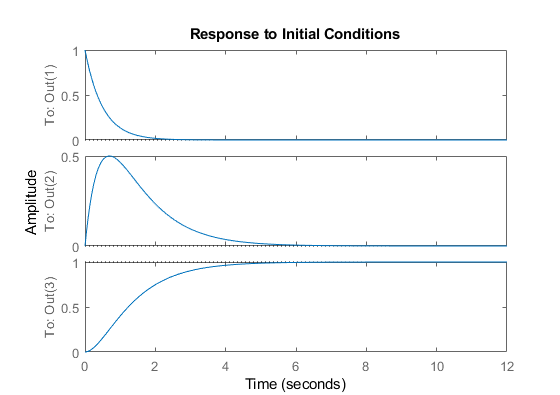
\includegraphics{ss_sim}










\end{document}
